The SI is structured as follows: first, we discuss the data used in our study and derive the regions' crop calendars in Sec.~\ref{si:MM}. Then, we give a comprehensive model description in Sec.~\ref{si:modDet}, before eventually providing details on the different scenarios discussed in the main text in Sec.~\ref{si:scen}.  

\section{Materials and Methods}
\label{si:MM}
Regional consumption, annual production, and ending stock data are derived from the Production,
Supply, and Distribution database of USDA's Foreign Agricultural Service
(USDA-PSD)\footnote{\url{https://apps.fas.usda.gov/psdonline}, accessed June, 2017.}.  For the
simulations presented in this study, we group the countries contained in the USDA-PSD database into
five agricultural regions. Four of them, EUR, FSU, NAF, and CPA, are the world's main wheat
producing regions, and the rest of the countries is lumped together in the ROW region. Country names
and the number of countries accounted for in the database have been changing over time.
Table.~\ref{tab:conGroup} shows the assignment of all (present as well as former) countries and
groups of countries (e.g., EUR-15) included in the database for the international trade years 1980
to 2016 to the five agricultural regions of this study.
\begin{table}[htbp]
  \caption{Grouping of countries into the five agricultural regions: European Union (EUR), Former Soviet Union (FSU), North Atlantic Free Trade countries (NAF), Centrally Planned Asia (CPA ), and rest of the world (ROW). Country names are stated as given in the USDA-PSD online database.}
  \label{tab:conGroup}
  \centering
    \begin{tabularx}{\textwidth}{lX}
      Region & Country\\
      \toprule
      \multirow{2}{*}{CPA} & China, Hong Kong, Democratic People's Republic of Korea, Mongolia, Singapore, Taiwan, Viet Nam\\
      \midrule
      \multirow{3}{*}{FSU} & Armenia, Azerbaijan, Belarus, Georgia, Kazakhstan, Kyrgyzstan, Republic of Moldova, Russian Federation, Tajikistan, Turkmenistan, Union of Soviet Socialist Republics (USSR), Ukraine, Uzbekistan\\
      \midrule
      \multirow{4}{*}{EUR} & Albania, Bosnia and Herzegovina, Bulgaria, Croatia, Cyprus, Czechia, EU-15, Estonia, European Union, Former Czechoslovakia, Hungary, Latvia, Lithuania, Republic of Macedonia, Malta, Norway, Poland, Romania,
        Serbia, Serbia and Montenegro, Slovakia, Slovenia, Switzerland, Socialist Federal Republic of Yugoslavia \\
      \midrule
            NAF & Canada, Mexico, United States\\
      \midrule
      \multirow{14}{*}{ROW}
             & Afghanistan, Algeria, Angola, Argentina, Australia, Bahrain, Bangladesh, Barbados, Benin, Bhutan, Plurinational State of Bolivia, Brazil, Burkina Faso, Cameroon, Chad, Chile, Colombia, Congo, The Democratic Republic of the Congo, Costa Rica, Cuba, Cote d'Ivoire, Dominican Republic, Ecuador, Egypt, El Salvador, Eritrea, Ethiopia, Fiji, Gabon, Ghana, Guatemala, Guinea, Guyana, Haiti, Honduras, India, Indonesia, Islamic Republic of Iran, Iraq, Israel, Jamaica, Japan, Jordan, Kenya, Republic of Korea, Kuwait, Lebanon, Lesotho, Liberia, Libya, Madagascar, Malawi, Malaysia, Mali, Mauritania, Mauritius, Morocco, Mozambique, Myanmar, Namibia, Nepal, New Zealand, Nicaragua, Niger, Nigeria, Oman, Pakistan, Panama, Papua New Guinea, Paraguay, Peru, Philippines, Rwanda, Saudi Arabia, Senegal, Sierra Leone, Somalia, South Africa, Sri Lanka, Sudan, Syrian Arab Republic, United Republic of Tanzania, Thailand, Togo, Trinidad and Tobago, Tunisia, Turkey, Uganda, United Arab Emirates, Uruguay, Bolivarian Republic of Venezuela, Yemen, Yemen (Aden), Yemen (Sanaa), Zambia, Zimbabwe\\
      \bottomrule
    \end{tabularx}
    %\addtabletext{MENA\ldots}
  \end{table}
  Nominal WM prices for US hard red winter wheat are taken from the Commodity Markets online
  database of the World Bank\footnote{http://www.worldbank.org/en/research/commodity-markets,
    accessed June, 2017.}, and real prices are obtained by deflating with the US All Urban Consumers
  price index (June 1983 = 100) provided by the US Bureau of Labor
  Statistics\footnote{https://www.bls.gov, accessed June, 2017.}. Further, the regional crop
  calenders, i.e., the percentage of production harvested in each time step is calculated by
  combining data on the harvesting season for winter wheat from \cite{SAC10} (interpolated dataset
  with 5\minute~by~5\minute~resolution) with harvested areas and yields for the year 2000
  taken from a global gridded, observational dataset \cite{MON08} (same resolution) obtained from
  remote sensing. For each grid cell, we assume that there is one harvest per year, which is normal
  distributed. In order to obtain the regional harvest distributions (Fig.~\ref{fig:crop_cal}), this
  distribution is weighted by the cell's production, and aggregated over each agricultural
  region. The model is implemented in python; the program code is available upon request.
\begin{figure}[htbp]
  \centering
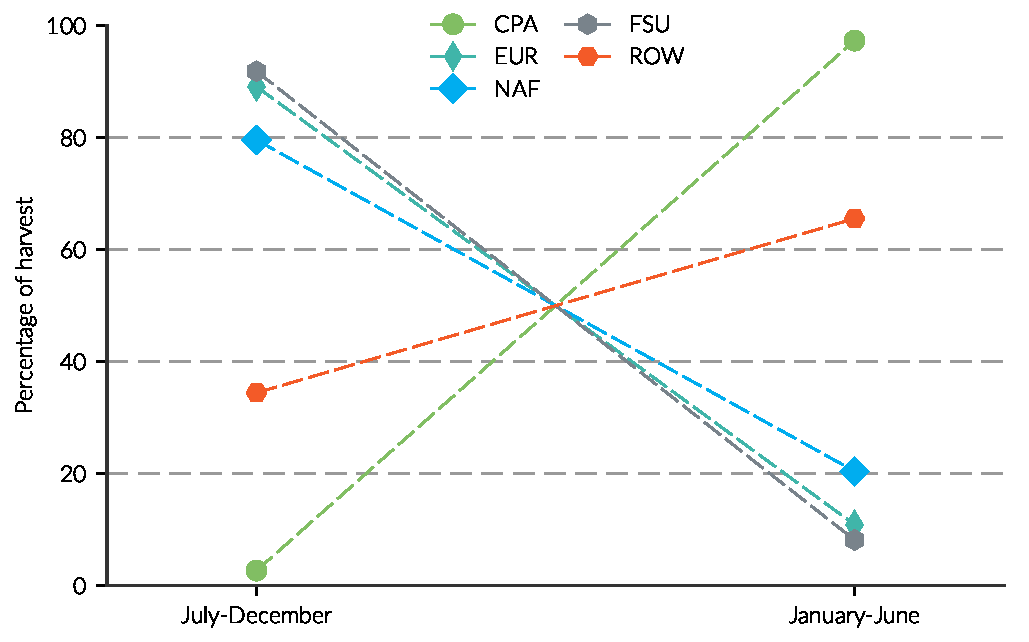
\includegraphics[width=.8\textwidth]{plots/crop_calendar/crop_cal_gridded}
\caption{Crop calendar for the five agricultural regions: European Union (EUR), Former Soviet Union (FSU), North Atlantic Free Trade countries (NAF), Centrally Planned Asia (CPA), rest of the world (ROW). The international trade year for wheat spans from July to June, in accordance with the USDA-PSD online database.}
  \label{fig:crop_cal}
\end{figure}

\section{Modeling details}
\label{si:modDet}
The subsequent section provide a comprehensive model description. First, we discuss the rationales
of the various economic agents in Sec.~\ref{si:econAgents}, before describing their interaction on
the WM in Sec.~\ref{si:market_dyn}. Then, we provide details on the implementation of stockkeeping
policies short-term market interventions in Sec.~\ref{si:trad_pol}, and, eventually, discuss the
initial conditions in Sec.~\ref{si:iniCond}. A summary of the exogeneous parameters used in the
simulations is provided in Tab.~\ref{tab:params}.
\begin{table}[htbp]
  \caption{Exogeneous parameters of the model used in the simulations if not indicated otherwise. $\langle\cdot\rangle_a$ denotes the temporal average of the last $a$ years. Regional parameters are identical for all regions if not states otherwise.}
  \label{tab:params}
  \centering
    \begin{tabular}{lll}
      Meaning & Symbol & Value \\
      \toprule
      No. of timesteps per year & $N$ & $2$\\
      Storage costs & $k_r$ & $20\USD/\Mt/\annum$\\
      Loss rate & $\rl_r$ & $3.5\%/\annum$\\
      Interest rate & $\gamma$ & $2.5\%/\annum$\\
      Maximum consumer price & $\Pmax_r$ & $435\USD$\\
      Price elasticity & $\ec$ & $0.4$\\
%      Demand elasticity & $\dce_r$ & in sim. demand set to hist. data\\
      Reference price & $\Pref$ & $90\USD$\\
      \midrule
      Capacity of strategical storage & $\Ismaxr$ & see Sec.~\ref{si:trad_pol}\\
      Strength of export restriction & $\erd_r$ & see Sec.~\ref{si:trad_pol}\\
      \midrule
      Center price of price band & -- & $\av{P}{15}$\\
      \bottomrule
    \end{tabular}
  \end{table}

\subsection{Economic agents}
\label{si:econAgents}
As described in the main text, the agricultural economic activities in each region $r\in R$
of the set of regions $R$ are described by three agents: a commercial storage holder, a
strategic storage holder, and a domestic consumer. Their rationales are detailed in the subsequent
paragraphs.

\paragraph*{Commercial storage holder}
We model the commercial storage holder of a region $r$ as a risk-neutral
bounded-rational agent. At each timestep $t$, the agent receives an amount of grain $h_r^t$
harvested in the region and then plans its WM supplies
$\bs y_r^t\equiv(y_r^0,\ldots,y_r^{N-1})^{\bot}$ by maximizing expected profit over the forecasting
period split into $N$ timesteps. Expected profit is calculated from the difference between expected
revenues and warehousing costs in this period reading
\begin{equation}
  \label{eq:exp_profit} \hPi_r(\bs y_r)\equiv
\sum_{n=0}^{N-1}\frac{\hP_r^n(y_r^n)\, y_r^n}{(1+\gamma)^n} -k_r\sum_{n=0}^{N-1}
n\, y_r^n.
\end{equation}
Here, $\hP_r^n$, $\gamma$, and $k_r$ denote the agent's expectation on the WM price at time $t+n$,
the interest rate, and the storage costs per timestep, respectively. The expected profit depends on
the agent's expectation on future WM prices. To form these expectations, the agent estimates (i) its
own impact on WM price, (ii) its own harvest in the next year, (iii) the WM supplies of its
competitors during this period, and (iv) WM demand. Here, we assume that all regional agents have
access to the same global supply and demand forecasts provided for instance by the Food and
Agricultural Agency (FAO) of the UN or by the quarterly Supply and Demand forecasts of the United
States Department of Agriculture (USDA) providing them with a foresight horizon of one year.

Having no precise knowledge on future WM supplies of its competitors and future demand side
stockholding policies, the agent assumes a simple iso-elastic dependence of WM price on WM supply
reading
\begin{equation}
  \label{eq:exp_WM_price}
P_r^n(y_r^n)\equiv \Pref \left(\frac{\hS_r^{R,n}+y_r^n}{\hD_n} \right)^{\frac{1}{\ec}},
\end{equation}
where $\Pref$, $\hS_r^{R,n}$, $\hD_n$, and $\ec$ denote a reference price, the agent's expectation
on the WM supply of its competitors, expected WM demand, and the price elasticity of WM supply,
respectively. The agent calculates $\hS_r^{R,n}$ by taking the supply forecast of the international
agency $\hS^n$ and subtracting its own expected contribution $\hs_r^n \hS^n$ yielding
\begin{equation}
  \label{eq:SROW}
  \hS^{R,n}_r \equiv (1- \hs_r^n) \hS^n.
\end{equation}
Here, we assume that the agent estimates its share $\hs_r^n$ on future WM supply by averaging over
its shares in the last 2 years. The global supply and demand forecasts, $\hS_n$ and $\hD_n$, are
derived from USDA production and domestic consumption data smoothed with a Savitzky-Golay filter
with a window size of 31 years (see Fig.~\ref{fig:supProd_and_cons}(global)).
\begin{figure}[htbp]
  \centering 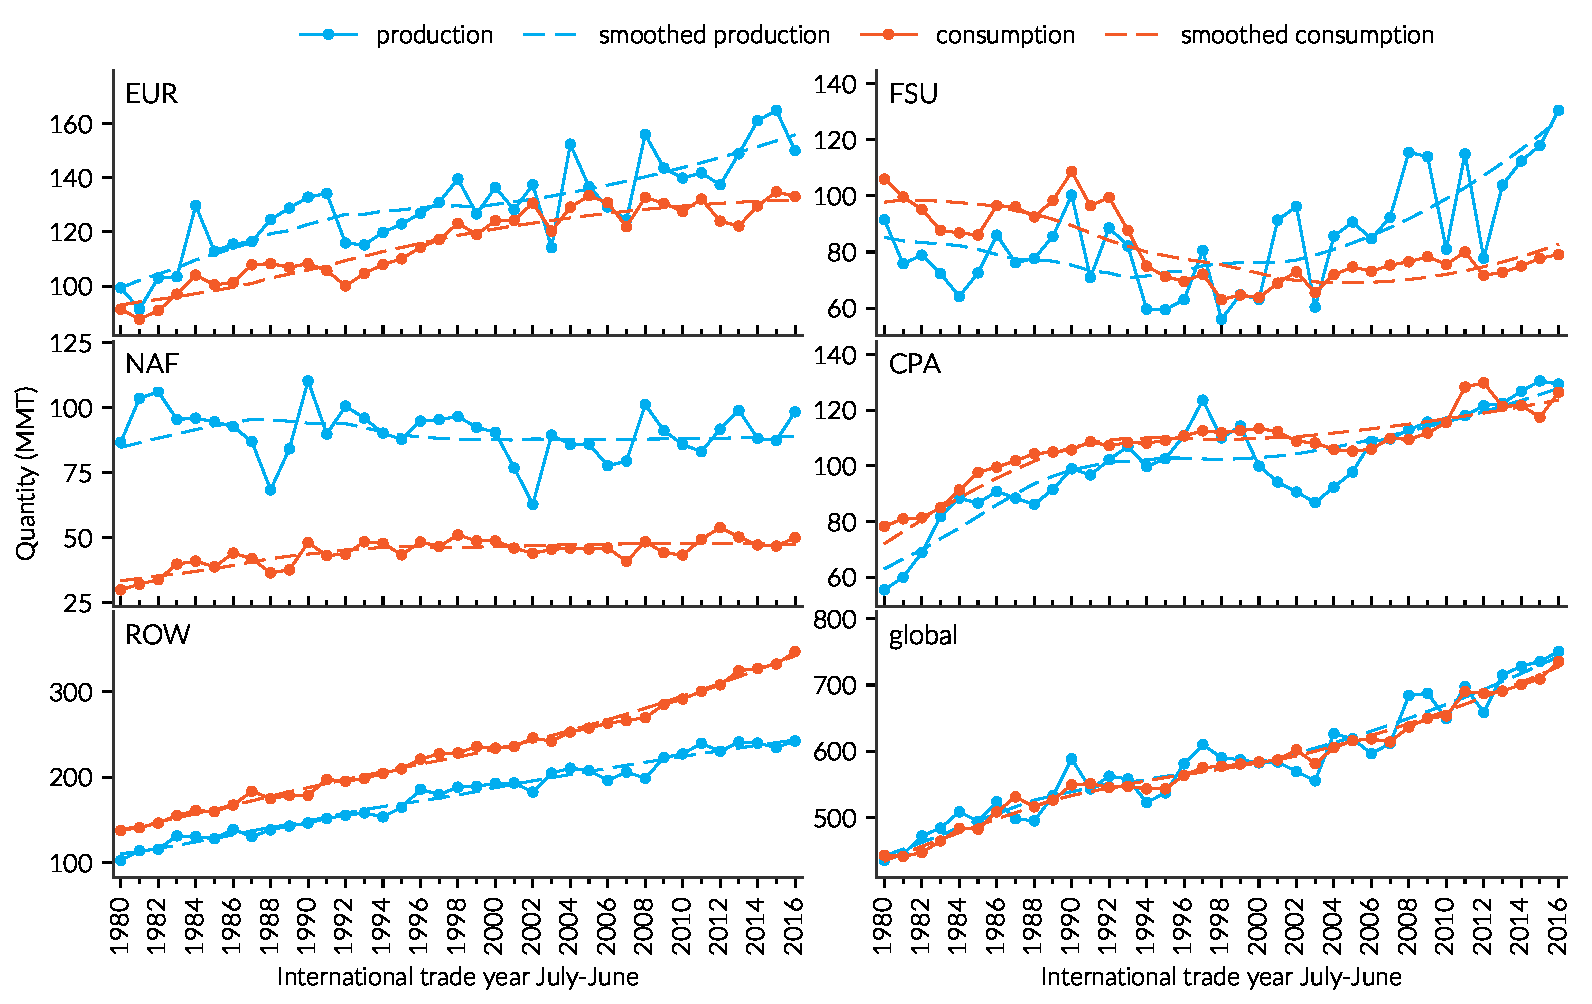
\includegraphics[width=.8\textwidth]{plots/USDA_supply_and_demand/prod_cons_1980_2016.pdf}
  \caption{Historical production and domestic consumption data as reported by USDA for the five main
    agricultural regions: European Union (EUR), Former Soviet Union (FSU), North Atlantic Free Trade
    Agreement countries (NAF), Centrally planned Asia (CPA), the rest of the world (ROW) as well
    as globally (global). Dashed lines indicated smoothed data used for the global supply and demand
    forecasts. The international trade year spans from July to June.}
  \label{fig:supProd_and_cons}
\end{figure}

Finally, the commercial storage holder obtains the optimal distribution of WM supplies $\yropt$ by
maximizing $\hPi_r$ over the forecast period under the constraints that (i) all supplies have to be
non-negative, (ii) they must not exceed its expected storage content, and (iii) export restrictions
may temporally limit the amount of grain it can sell on the WM yielding the following constraint
optimization problem
\begin{subequations}
\label{eq:yopt}
\begin{align}
  &\yropt \equiv \underset{\bs y_r}{\argmax}\left[\hPi_r(\bs y_r)\right],\text{ subject to}\\
  &y_r^n \geq 0\,\, \forall n\,\wedge\, \bs L\cdot \bs y_r \leq (1-\erd_r)\left[I_r\mathbb{I} + \bs L \cdot\bs \hh_r\right]\label{subeq:capac_constraint}.
\end{align}
\end{subequations}
Here, $\bs L$ denotes a lower triangular matrix of ones, `$\cdot$' is the scalar product, and
$\erd_r\in[0,1]$ is the share of the agent's expected storage content that it cannot sell on the WM
in case of a regional export restriction. Further, $\mathbb{I}$, $I_r$ denote the identity vector,
and the agent's storage content, respectively. For simplicity, we assume that the agent's estimates
on its own upcoming harvests $\bs \hh_r$ within the forecast period are perfect.

\paragraph*{Strategic storage holder}
The strategic storage holder aims at providing food security for the region's domestic
consumption. In contrast to the commercial storage holder, the strategic storage holder aims to
assure a certain inventory level instead of maximizing profit. We assume that its demand decreases
linearly with price (see also \cite{SCH17} for a detailed discussion)
\begin{equation}
  \label{eq:D_r}
  D_r(P)\equiv\max\left[\Dmax_r\Big(1 - \frac{P}{\Pmax_r}\Big),0\right],
\end{equation}
where $\Dmax_r\equiv \Ismaxr - I_r^{s,t-1}$ is the available storage space given by the difference
between total storage capacity $\Ismaxr$, an exogeneous measure for the region's target inventory
level, and $I_r^{s,t-1}$, the inventory carry over from the last time step. Further, $\Pmax_r$
denotes the maximum price up to which the agent is willing to purchase a non-zero amount.

\paragraph*{Domestic consumer}
The third agent type represents the region's domestic consumption, which is assumed to depend
iso-elastically upon WM price. We assume that domestic consumers do not directly purchase grain from
the WM, but refer to the region's strategic storage. Consequently, this agent's consumption is
limited by the content of the strategic storage, $I_r^{s,t-1}+D_r(P)$. Unless stated otherwise,
annual regional consumption is fixed to the values reported by USDA. However, for some simulations,
we assume an iso-elastically dependence of regional consumption upon WM price
\begin{equation}
  \label{eq:C_r}
 C_r(P)\equiv \min\left[\Cref_r\left(\frac{P}{\Pref_r} \right)^{\dce_r},I_r^{s,t-1}+D_r(P)\right],
\end{equation}
where $\Cref_r\equiv\Cref_r(\Pref_r)$ denotes the reference level of domestic consumption estimated
from past values of domestic consumption, and $\dce_r$ denotes the region's demand elasticity. The
latter may vary among regions, which accounts for their different dependencies upon the modeled
crop.

\subsection{Market dynamics}
\label{si:market_dyn}
We assume that the market clears in each timestep, and the equilibrium price $\Peq$ is determined by
equating WM supply $S\equiv \sum_{r\in R} \yropt$ and WM demand $D(P)\equiv \sum_{r\in R}D_r(P)$,
i.e., we obtain $\Peq$ by solving $S=D(\Peq)$ for $\Peq$. Next, the inventories of commercial and
strategic storage holders are updated according to the rules
\begin{align}
  \label{eq:stor_update}
  I_r &= (1-\rl_r)\,I_r^{t-1} -y_r + h_r, \\
  \Isr &= (1-\rl_r)\,I_r^{s,t-1} + D_r(\Peq)-C_r(\Peq),
\end{align}
where $\rl_r$ is the loss rate for storing grain, $I_r^{t-1}$ and $I_r^{s,t-1}$ denote the
carry-over stocks of region $r$'s commercial and strategic storage holders, respectively, and $h_r$
denotes the region's harvest in the present timestep. The loss rates $\rl_r$ for crop spoilage are
identical for all regions as well as for the international reserve. They are estimated from best fit
of the ending stocks for the scenario accounting only for regional production and consumption
variabilities (see Sec.~\ref{si:scen} for details).

% \paragraph*{Trade policies}
% We consider two types of regional trade policies: changes in strategic
% stockholding policies and export restrictions. A stockholding policy in region
% $r$ is modeled by varying $\Ismaxr$ (cf.~Eq.~(\ref{eq:D_r})), which is a proxy
% for the region's target inventory level. Further, we assume that other important
%   consumer side policy measures such as import subsidies can be also represented
%   by changes in $\Ismaxr$.. These policies determine the stocks-to-use (stu)
% ratio, which is perceived as the optimal tradeoff between food security in times
% of scarcity and costs in normal times. Consequently, reported stu-ratios,
% calculated from the ratio of ending stocks and domestic consumption, differ
% significantly among regions, and they change over time (see
% Fig.~\ref{fig:stuRatios} in SI). For instance, the abrupt decline of ending
% stocks in the NAF region between $1986$ and $1988$ marks the transition from
% governmentally managed stocks to a market-oriented stockholding scheme
% \cite{WES99} (see ending stocks and stu-ratio for NAF region in
% Fig.~\ref{fig:Fig2} and Fig.~\ref{fig:stuRatios} in SI, respectively). We use
% these regional changes in stu-ratios as proxies for regional changes in the
% demand for strategic stockholding expressed by $\Ismaxr$ in the model
% (cf.~Eq.~(\ref{eq:D_r})).

% Further, major reported national export restrictions are implemented by non-zero
% values of $\erd_r$ (cf.~Eq.~(\ref{subeq:capac_constraint})). Since export
% restrictions are short-term policy measures in times of crises, we assume that
% agents cannot foresee the onset of export restrictions nor their revocation. The
% commercial storage holder of the region imposing the export restriction
% therefore assumes that, once imposed, the restriction will remain in place for
% the whole foresight period.

% Since it is not possible to derive the absolute values of both $\Ismaxr$ and
% $\erd_c$ directly from the trade data, these parameters are determined by best
% fit of simulated prices and regional ending stocks with the reported
% ones. Details on the implementation of policies are discussed in
% Sec.~\ref{si:trad_pol} of the SI and Tab.~\ref{tab:tradPol} lists the policies
% that we account for, their timing, and reporting sources.

% \paragraph*{International reserve}
% \label{sec:int_reserve}
% The price stabilization reserve is a measure designed to reduce price volatility
% by stabilizing prices within a certain price band $\Peq\in[\Pfl,\Pceil]$
% centered around a center price $\Pc$, representing market fundamentals. The
% price band is limited from below by a floor price $\Pfl$ and from above by a
% ceiling price $\Pceil$. If $\Peq$ drops below $\Pfl$, the reserve is filled by
% purchases from the WM until $\Peq$ increases above $\Pfl$ or the reserve is
% filled to its capacity. If $\Peq$ exceeds $\Pceil$, grain is released from the
% reserve onto the market until either $\Peq$ drops below $\Pceil$ or the reserve
% is depleted.


\subsection{Policies}
\label{si:trad_pol}
In this section, we discuss the calibration of the model with respect to the capacities of the
strategic inventories $\lbrace\Ismaxr\rbrace_r$, which are proxies for the regions' target demand
for strategic stockkeeping, and the factors $\lbrace\erd_c\rbrace_r$, which are measures for the
strengths of regional export restrictions. As discussed in the main text, we use reported changes of
a region $r$'s annual stu-ratio as a proxy for changes in $\Ismax_r$.  Further, we assume that other
measures for the protection of domestic consumers as for instance import subsidies can be also
represented by changes in the $\lbrace \Ismax_r \rbrace_r$.

To obtain $\Ismax_r$ for region $r$'s strategic storage holder, from the time series of the region's
reported stu-ratio $\rstu_r$, we first determine intervals in which this ratio does not vary
significantly. In these intervals, we then set $\Ismaxr$ to a multiple $m_r$ of the mean stu-ratio
in this interval $\avrstu_r$ multiplied by the region's mean domestic consumption in the last three
years and its mean expected consumption within the foresight period $\langle C_r\rangle_{3+1}$,
i.e., $\Ismaxr$ reads
\begin{equation}
  \label{eq:Ismaxr}
  \Ismaxr \equiv m_r\avrstu_r \langle C_r\rangle_{3+1}.
\end{equation}
\begin{figure}[htbp]
  \centering
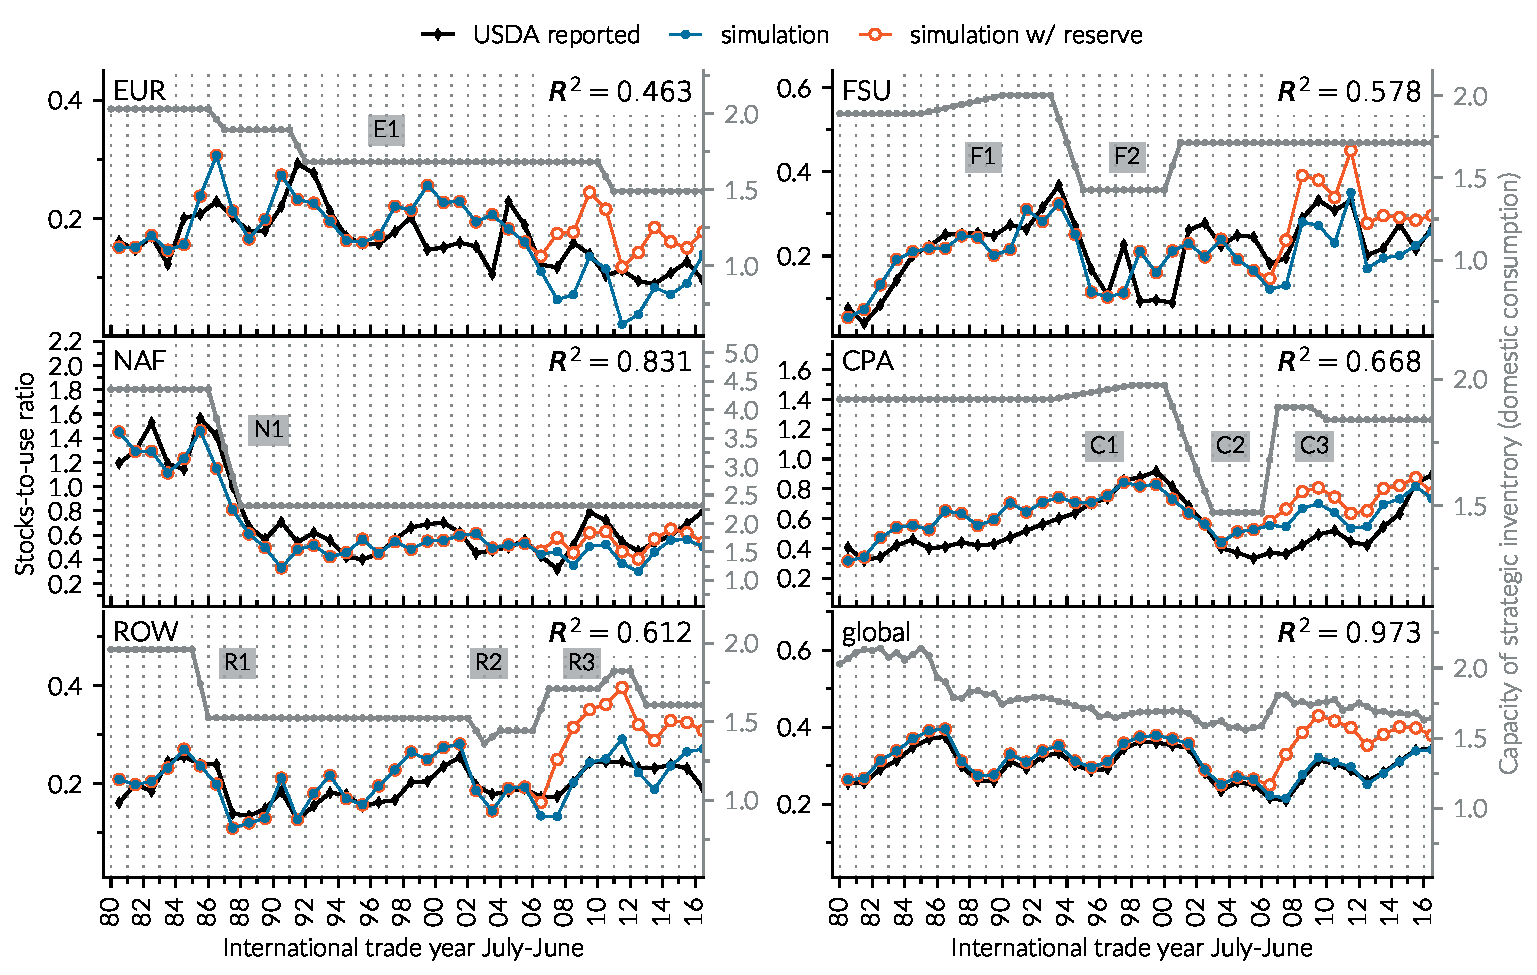
\includegraphics[width=.8\textwidth]{plots/full/Stocks-to-use_ratio_1980_2017}
\caption{Stocks-to-use (stu) ratios for the five economic regions: European Union (EUR), Former
  Soviet Union (FSU), North Atlantic Free Trade countries (NAF), Centrally Planned Asia (CPA), rest
  of the world (ROW), as well as globally (global). Black diamonds, blue dots, and open orange
  circles, indicate ending stocks as reported by USDA, for the historical scenario without and with
  international reserve, respectively. Squared Pearson correlation coefficients $R^2$ denote the
  correlation between reported stu-ratios and the simulation without reserve. Small gray dots
  ($\secnd$ y-axes) denote the capacity of the regions's strategic reserves in multiples of domestic
  consumptions (cf.~ Eq.~(\ref{eq:Ismaxr})). Capacity changes result from the policies (labels in
  gray rectangles) listed in Tab.~\ref{tab:tradPol}. Parameters are as in Tab.~\ref{tab:params}.}
  \label{fig:stuRatios}
\end{figure}
Policy changes are represented by linearly connecting the intervals of constant $\avrstu_r$. The
absolute level of $\Ismax_r$, i.e., the multiple $m_r$, is determined by the best fit of modeled
prices and regional ending stocks with their observed counterparts. Fig.~\ref{fig:stuRatios} depicts
regional observed annual stu-ratios (black diamonds) as well as the simulated stu-ratios for the
scenarios without (blue dots) and with (open orange circles) international reserve; the second
y-axes depict the products of the multiples $m_r$ and fitted stu-ratios $\rstu_r$. Further, we
have verified that all policies accounted for in our simulations are reported in the literature. In
Fig.~\ref{fig:stuRatios}, these policies are labeled by gray rectangles with one-letter codes of the
economic regions issuing the policy followed by ascending numbers. Descriptions of policies, their
timing, and reporting sources are summarized in Tab.~\ref{tab:tradPol}.

\paragraph*{Export restriction}
Export restrictions in a region $r$ are modeled by non-zero values of $\erd_r$. We first identified
the major export restrictions by a literature research. The specific value that $\erd_r$ assumes
when a export restriction is in place is determined by the best fit of simulated prices and ending
stocks with their reported counterparts. All export restrictions accounted for in the simulations,
their timing, and the reporting literature sources are listed in Tab.~\ref{tab:tradPol}.
\begin{table}[ht]
  \caption{Reported policies taken into account in the simulations to reproduce historical prices and ending stocks. The lower part of the table describes export restrictions. The parameter values of $\erd_R$ (cf. Eq.~(\ref{subeq:capac_constraint})) used in the simulations are given in rounded brackets.}
  \label{tab:tradPol}
  \centering
    \begin{tabularx}{\textwidth}{llX}
      Event label & Time period & Description \\
      \toprule
      \multirow{2}{*}{E1} & \multirow{2}{*}{early  90s -- mid 00s}
                          & Gradual reduction of governmental stocks in EU to comply with Uruguay Round of WTO \cite{WB12}.\\
      \midrule
      \multirow{1}{*}{F1} & \multirow{1}{*}{80s} & Increase in strategical stocks in USSR \cite{AND08}.\\
      \addlinespace
      \multirow{3}{*}{F2} & \multirow{3}{*}{early 90s -- early 00s} & Decline and subsequent recovery of stocks due to restructuring of agricultural production and trade after breakdown of USSR \cite{AND08, LIE13}.\\
      \midrule
      \multirow{2}{*}{N1} & \multirow{2}{*}{1985} & Reduction of governmental stocks in US during transition to market-oriented stockholding policies \cite{WES99}.\\
      \midrule
      \multirow{2}{*}{C1} & \multirow{2}{*}{90s}& Accumulation of governmental stocks due to strong producer support \cite{FAO99,HSU01}.\\
      \addlinespace
      \multirow{2}{*}{C2} & \multirow{2}{*}{1999 -- 2004} & Decrease of stocks due to grain marketing and reserve reform in the course of China's WTO accession \cite{DAW09,HSU01}.\\
      \addlinespace
      \multirow{1}{*}{C3} & \multirow{1}{*}{2008 \& 2011} & Unusual purchases by China to restock inventories \cite{TRO11}.\\
      \midrule
      \multirow{2}{*}{R1} & \multirow{2}{*}{90s} & Reduction of public stockholding in OECD countries to comply with Uruguay Round of WTO \cite{WB12}.\\
      \addlinespace
      \multirow{2}{*}{R2} & \multirow{2}{*}{2003 -- 2004} & Unusual high exports of India and Brazil due to record stock levels\footnote{USDA's PSD online database \url{https://apps.fas.usda.gov/psdonline}, accessed June 2017}.\\
      \addlinespace
      \multirow{2}{*}{R3}
            & \multirow{1}{*}{2008} & Unusual purchases India, Iran, Mexico, MENA \cite{HEA08}.\\
            & \multirow{1}{*}{2011} & Build-up of food security stocks in MENA \cite{TRO11}.\\
      \midrule\midrule
            & \multirow{1}{*}{10/2006 -- 5/2007}  & Export quota Ukraine \cite{SHA11} ($\erd_{\FSU}=0.1$).\\
            & \multirow{1}{*}{6/2007 -- 5/2010}  & Export (quasi) ban Ukraine \cite{SHA11} ($\erd_{\FSU}=0.2$).\\
            & \multirow{1}{*}{8/2010 -- 4/2011}  & Export quota Ukraine \cite{SHA11} ($\erd_{\FSU}=0.15$).\\
       & \multirow{1}{*}{4/2008 -- 10/2008} & Export ban Kazakhstan \cite{SHA11} ($\erd_{\FSU}=0.2$).\\
       & \multirow{1}{*}{8/2010 -- 10/2011}  & Export ban Russia \cite{TRO11,GrainChain12} ($\erd_{\FSU}=0.15$).\\
      \bottomrule
    \end{tabularx}
 \end{table}
% \afterpage{\clearpage}

\subsection{Initial conditions}
\label{si:iniCond}
For calibration, it is convenient to run the model from a steady state close to the state given by
the annual production and consumption data of the simulation's start year. Note that, in general,
global annual production and consumption do not match, and the simulation's start year therefore
usually does not constitute a steady state of the dynamical system.

We construct the initial steady state by taking the regional productions of the start year, and
modifying regional consumption such that global consumption equals global production. For that, we
first determine the share of global consumption that each region has in the start year. Then,
regional consumptions are determined by multiplying these shares with the global production of the
start year.

\paragraph{Inventory of competitive storage holder}
We assume that in the initial steady state, the commercial storage holder of a region does not carry
over any inventory from one local agricultural year to the next, i.e, for biannual time steps, the
agent sells in average one half of its annual harvest in each time step on the WM. Note that, if the
local agricultural year differs from the international trade year (July to June), the agent can
nevertheless have finite ending stocks at the end of the latter, i.e, in June. Thus, the competitive
storage holders of EUR, FSU, and NAF, which have their harvest maximums in the first semester the
international trade year have zero ending stocks. In contrast to the competitive storage holders of
CPA and ROW, which have their harvest maximums in the second semester of the international trade
year and therefore have finite ending stocks. Summing up, ending stocks of the strategical storage
holders in the steady state read
\begin{equation}
  \label{eq:ES_strat_stor}
  I_r^{\star,2}\equiv\begin{cases}
    0, & \text{for }r\in[\EUR, \FSU, \NAF],\\
    \hrstar(\nu_{h,r}^{\star,2}-\frac{1}{2}), & \text{for }r\in[\CPA,\ROW],
  \end{cases}
\end{equation}
where $\hrstar$ and $\nu_{h,r}^{\star,2}$ denote region $r$'s harvest in the start year of the
simulation and the fraction harvested in the second semester of the international trade year,
respectively.

\paragraph{Inventory of strategical storage holder}
We assume that in the initial steady state the strategical storage holder's inventory content
remains constant, i.e., in each time step, the amount of grain purchased on the WM by region $r$'s
strategical storage holder equals the domestic consumption in this region. Thus, by taking the
ending stocks reported for the simulation's start year $I_r^{\sigma,\star,2}$ and subtracting the
ending stock of $r$'s competitive storage holder $I_r^{\star,2}$, we may obtain the ending stocks of
$r$'s strategical storage holder as
\begin{equation}
  \label{eq:ES_strat}
 I^{s,\star,2}_r\equiv I_r^{\sigma,\star,2} - I_r^{\star,2}.
\end{equation}
Next, we calculate the inventory size needed to ensure that $r$'s strategical storage holder
purchases on the WM equal $r$'s consumption $\starC_r\equiv \starC_r(\starP)$ in the steady
state. Here, $\starP$ denotes the WM price in the steady state, which is set to the WM price in the
first semester of the simulation's start year. For that, we equate $\starC_r$ to the demand of $r$'s
strategic storage holders, which reads according to Eq.~(\ref{eq:D_r})
\begin{equation}
  \label{eq:starCr}
  \starC_r = (\starIsmax_r - I_r^{s,\star,2}) \left(1-\frac{\starP}{\starPmax_r} \right).
\end{equation}
Solving the above equation for $\starIsmax_r$ then yields
\begin{equation}
  \label{eq:IrmaxIni}
  \starIsmax_r \equiv \frac{\starC_r}{1 - \starP/\Pmax_r}  + I_r^{s,\star,2}.
\end{equation}
Eventually, we set the spoilage rate equal to zero ($r^l=0$) in the steady state.

% \section{Country grouping}
% \label{si:country_grouping}
% For the simulations presented in this study, we group the countries contained in
% the USDA-PSD database into five agricultural regions. Four of them, EUR, FSU,
% NAF, CPA, are the main wheat producing regions, and the rest of the countries is
% lumped together in the ROW region. Country names and the number of
% countries accounted for in the database have been changing over time.
% Table.~\ref{tab:conGroup} shows the assignment of all (present as well as
% former) countries and group of countries (e.g., EUR-15) included in the database
% for the years $1980$ to $2016$ to the five agricultural regions of this study.
% \begin{table}[htbp]
%   \caption{Grouping of countries into the five agricultural regions: EUR (Europe 28), FSU (Former Soviet Union), NAF (North Atlantic Free Trade Agreement countries), CPA (Centrally Planned Asia), ROW (rest of the world). Country names are stated as given in the USDA-PSD online database.}
%   \label{tab:conGroup}
%   \centering
%     \begin{tabularx}{\textwidth}{lX}
%       Region & Country\\
%       \toprule
%       \multirow{2}{*}{CPA} & China, Hong Kong, Democratic People's Republic of Korea, Mongolia, Singapore, Taiwan, Viet Nam\\
%       \midrule
%       \multirow{3}{*}{FSU} & Armenia, Azerbaijan, Belarus, Georgia, Kazakhstan, Kyrgyzstan, Republic of Moldova, Russian Federation, Tajikistan, Turkmenistan, Union of Soviet Socialist Republics (USSR), Ukraine, Uzbekistan\\
%       \midrule
%       \multirow{4}{*}{EUR} & Albania, Bosnia and Herzegovina, Bulgaria, Croatia, Cyprus, Czechia, EU-15, Estonia, European Union, Former Czechoslovakia, Hungary, Latvia, Lithuania, Republic of Macedonia, Malta, Norway, Poland, Romania,
%         Serbia, Serbia and Montenegro, Slovakia, Slovenia, Switzerland, Socialist Federal Republic of Yugoslavia \\
%       \midrule
%             NAF & Canada, Mexico, United States\\
%       \midrule
%       \multirow{14}{*}{ROW}
%              & Afghanistan, Algeria, Angola, Argentina, Australia, Bahrain, Bangladesh, Barbados, Benin, Bhutan, Plurinational State of Bolivia, Brazil, Burkina Faso, Cameroon, Chad, Chile, Colombia, Congo, The Democratic Republic of the Congo, Costa Rica, Cuba, Cote d'Ivoire, Dominican Republic, Ecuador, Egypt, El Salvador, Eritrea, Ethiopia, Fiji, Gabon, Ghana, Guatemala, Guinea, Guyana, Haiti, Honduras, India, Indonesia, Islamic Republic of Iran, Iraq, Israel, Jamaica, Japan, Jordan, Kenya, Republic of Korea, Kuwait, Lebanon, Lesotho, Liberia, Libya, Madagascar, Malawi, Malaysia, Mali, Mauritania, Mauritius, Morocco, Mozambique, Myanmar, Namibia, Nepal, New Zealand, Nicaragua, Niger, Nigeria, Oman, Pakistan, Panama, Papua New Guinea, Paraguay, Peru, Philippines, Rwanda, Saudi Arabia, Senegal, Sierra Leone, Somalia, South Africa, Sri Lanka, Sudan, Syrian Arab Republic, United Republic of Tanzania, Thailand, Togo, Trinidad and Tobago, Tunisia, Turkey, Uganda, United Arab Emirates, Uruguay, Bolivarian Republic of Venezuela, Yemen, Yemen (Aden), Yemen (Sanaa), Zambia, Zimbabwe\\
%       \bottomrule
%     \end{tabularx}
%     %\addtabletext{MENA\ldots}
%   \end{table}

\FloatBarrier

% \section{Crop calendar}
% \label{si:crop_cal}
% Figure~\ref{fig:crop_cal} depicts the crop calendar for the five agricultural regions listed in Tab.~\ref{tab:conGroup} as obtained by the method discussed in the Materials and Methods section of the main text.

%\clearpage
\section{Scenarios}
\label{si:scen}
In this section, we describe the different scenarios discussed in the main text.

\subsection{Trends only}
\begin{figure}[htbp]
\centering 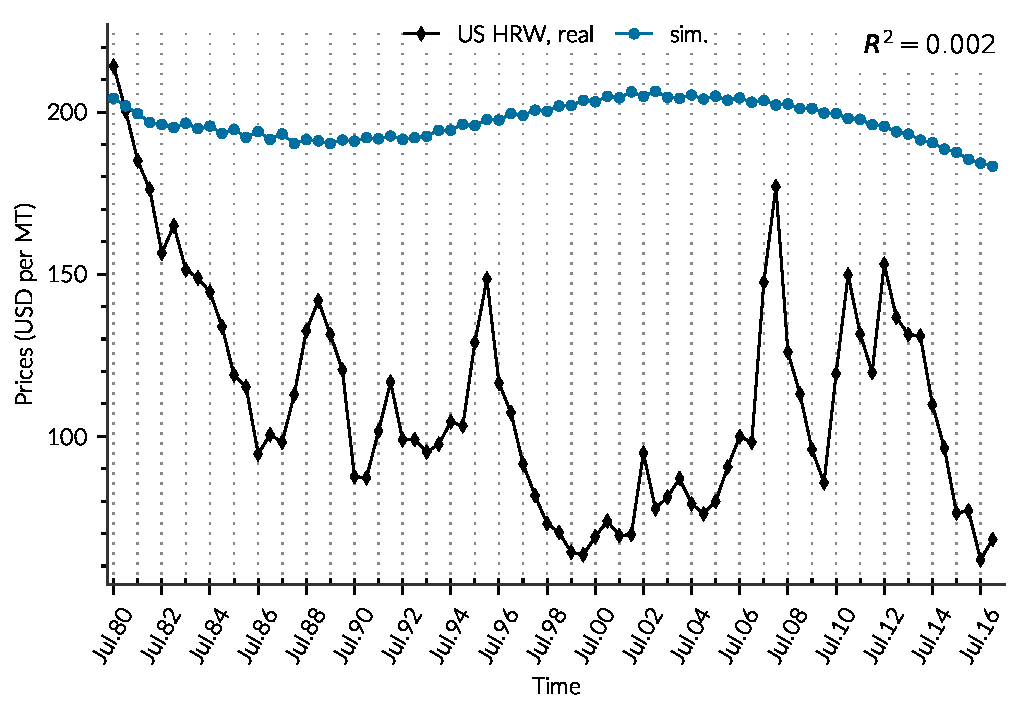
\includegraphics[width=.8\textwidth]{plots/trends_only/pric1980_2017}
\caption{Prices for the scenario accounting only for long-term changes in regional production and
  consumption. Black diamonds and blue dots indicate real and simulated wheat prices,
  respectively. The squared Pearson correlation coefficient $R^2$ denotes the correlation between
  reported and simulated prices. Parameters are as in Tab.~\ref{tab:params}.} %
  \label{fig:trendsOnly}
\end{figure}
\begin{figure}[ht]
  \centering 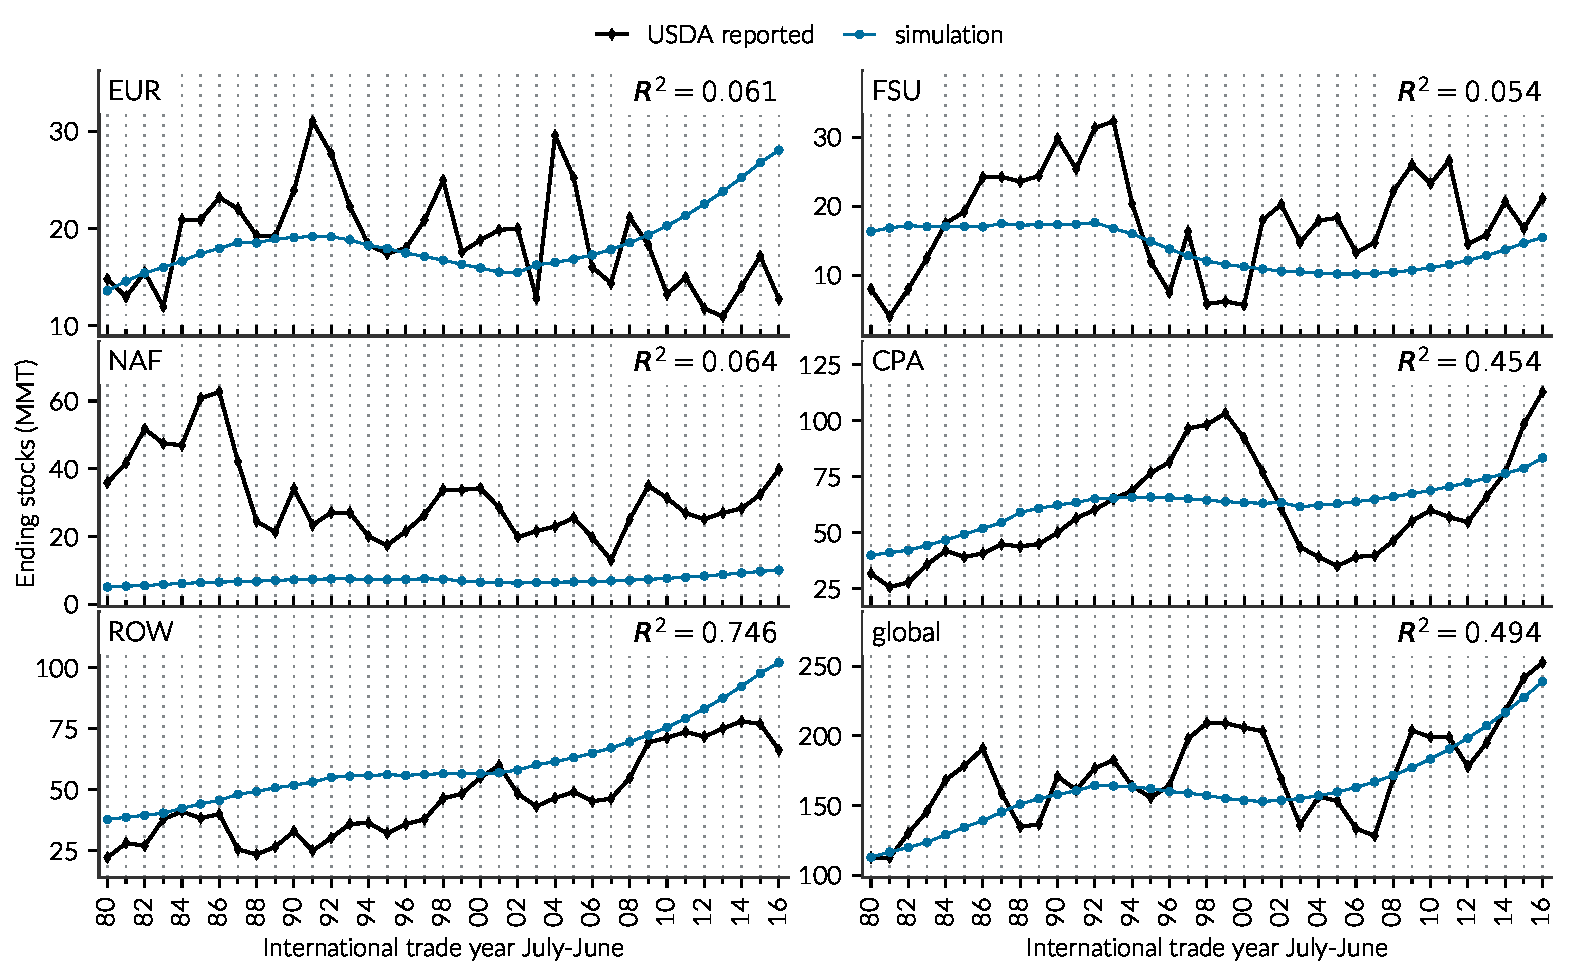
\includegraphics[width=.8\textwidth]{plots/trends_only/Ending_stocks__MMT__1980_2017}
  \caption{Regional ending stock for the scenario accounting only for long-term regional production
    and consumption trends. Reported and simulated ending stocks are denoted by black diamonds and
    blue dots, respectively. Squared Pearson correlation coefficients $R^2$ denote the correlation
    between reported and simulated ending stocks. Regions are the same as in Tab.~\ref{tab:conGroup}.}
  \label{fig:stocks_trendsOnly}
\end{figure}
This scenario accounts only for long-term regional production and consumption trends. As model
input, the smoothed production and domestic consumption time series of
Fig.~\ref{fig:supProd_and_cons} are used. The size of the strategic inventory in each region $r$ are
chosen to be a multiple of the temporal average of the region's mean domestic consumption in the
last three years and its mean expected consumption within the foresight period
$\langle C_r\rangle_{3+1}$ (cf. Eq.~(\ref{eq:Ismaxr})). Since the scenario does not take any
regional policies into account, the same multiple is chosen for all regions.  In the initial steady
state, first $\langle C_r\rangle_{3+1}$ is set to the adjusted domestic regional consumption
described in Sec.~\ref{si:iniCond}. Then, we calculate the global capacity of strategic inventories
$\starIsmax$ by summing Eq.~(\ref{eq:IrmaxIni}) over all regions. The common multiple is then set to
$\starIsmax/\langle C\rangle_{3+1}$, where $\langle C\rangle_{3+1}$ denotes the temporal average of
global domestic consumption.

It is worthy to note that the slight zigzagging of simulated prices in
Fig.~\ref{fig:trendsOnly} results from the finite costs for storage keeping. In this scenario,
expected consumption and world market supply are nearly constant over the foresight periods of the
competitive storage holders. Therefore, the storage holders decide to sell in the first semester of
their local agricultural years more grain on the WM than in the second semester. Because the
majority of wheat is produced in the Northern Hemisphere, more wheat is sold on the WM during the
harvesting season in the Northern Hemisphere (July-December) causing the periodical price drops.


\subsection{Production \& consumption variability}
\begin{figure}[htbp]
  \centering
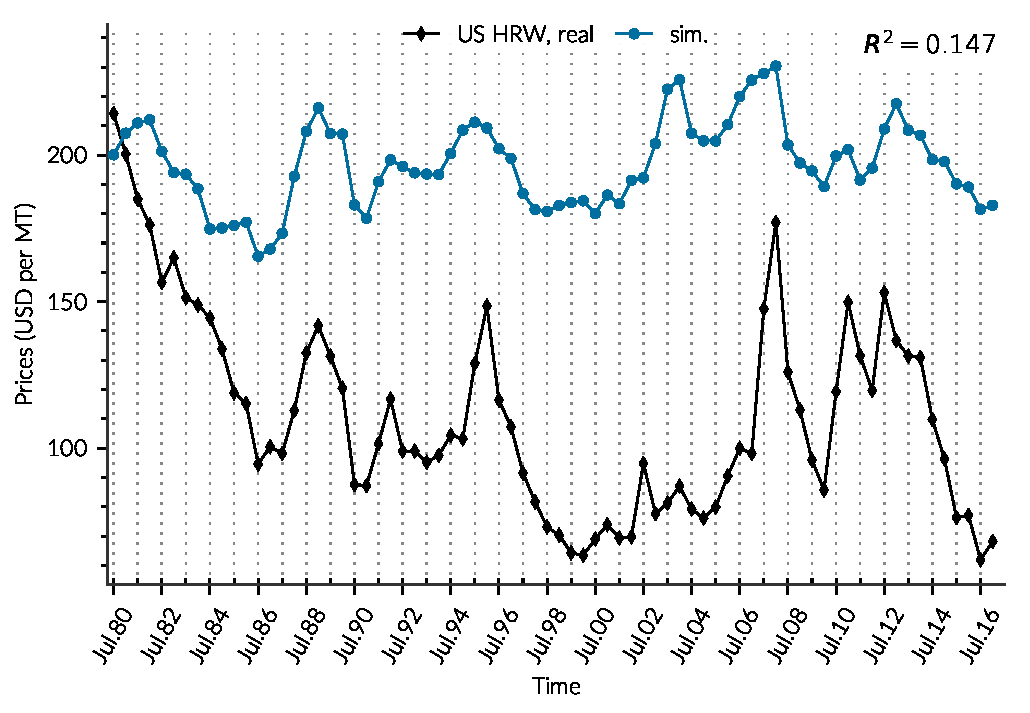
\includegraphics[width=.8\textwidth]{plots/baseline/pric1980_2017}
\caption{Prices for the scenario accounting for regional production and consumption
  variabilities. Black diamonds and blue dots indicate real wheat prices and simulated
  prices, respectively. The squared Pearson correlation coefficient $R^2$ denotes the correlation
  between reported and simulated prices. Parameters are as in Tab.~\ref{tab:params}.} %
  \label{fig:baseline}
\end{figure}
\begin{figure}[htbp]
  \centering 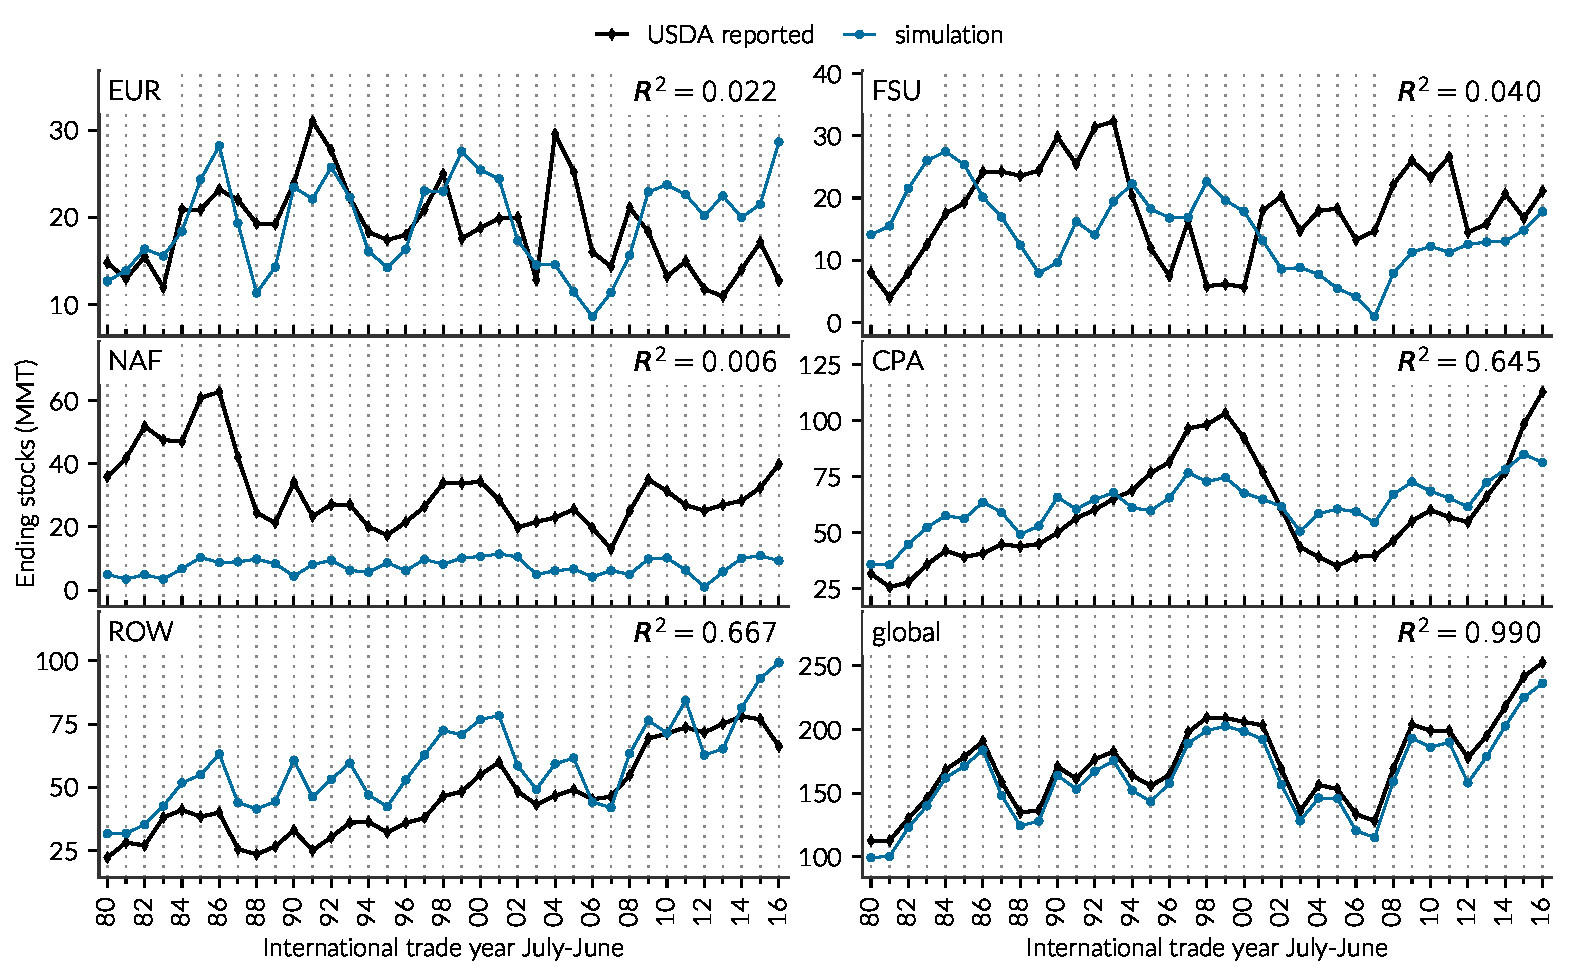
\includegraphics[width=.8\textwidth]{plots/baseline/Ending_stocks__MMT__1980_2017}
  \caption{Regional ending stock for the scenario accounting for production and consumption
    variabilities. Reported and simulated ending stocks are denoted by black diamonds and blue dots,
    respectively. Squared pearson correlation coefficients $R^2$ denote the correlation between
    reported and simulated ending stocks. Regions are the same as in Tab.~\ref{tab:conGroup}.}
  \label{fig:stocks_baseline}
\end{figure}
This scenario accounts for annual variability in production and domestic consumption (see production
and domestic consumption time series in Fig.~\ref{fig:supProd_and_cons}). Since no policies are
taken into account, the size of the strategic inventories are chosen as for the `trends only'
scenario.

% \FloatBarrier

\subsection{No policies from 2006 onwards}
\begin{figure}[htbp]
\centering  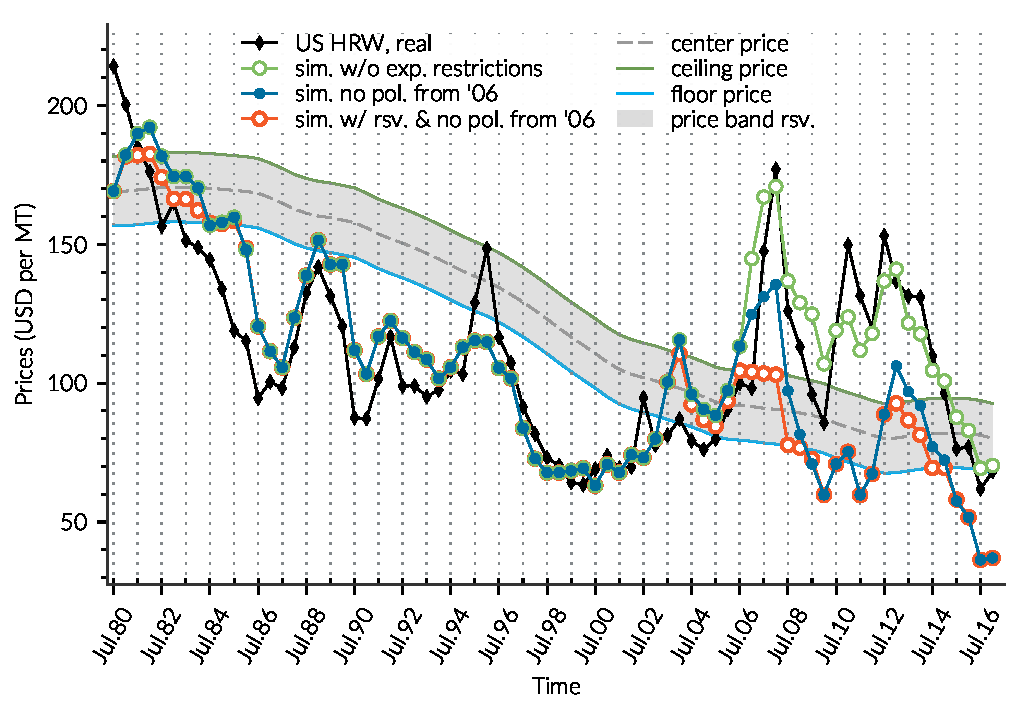
\includegraphics[width=.8\textwidth]{plots/no_policies_after_2006/pric1980_2017}
\caption{Prices for the scenarios without export restrictions and without policy interventions from
  2006 onwards. Black diamonds, green dots, blue dots, and open orange circles indicate real wheat
  prices, simulated prices for the scenario without export restrictions as well as the scenario
  without policy interventions from 2006 onwards (without and with an international reserve with a
  capacity of 30\mmt), respectively. The gray shaded area indicates the price band of the
  international reserve; the reserve is re-stocked (released) if prices drop below (increase above)
  the floor price (thin light-blue line) (ceiling price (thin green line)). The price band has a width of 25\USD~and spans around the 15-years running mean (gray dashed line). Parameters are as in Tab.~\ref{tab:params}.}
  \label{fig:prices_small_res}
\end{figure}
\begin{figure}[htbp]
  \centering 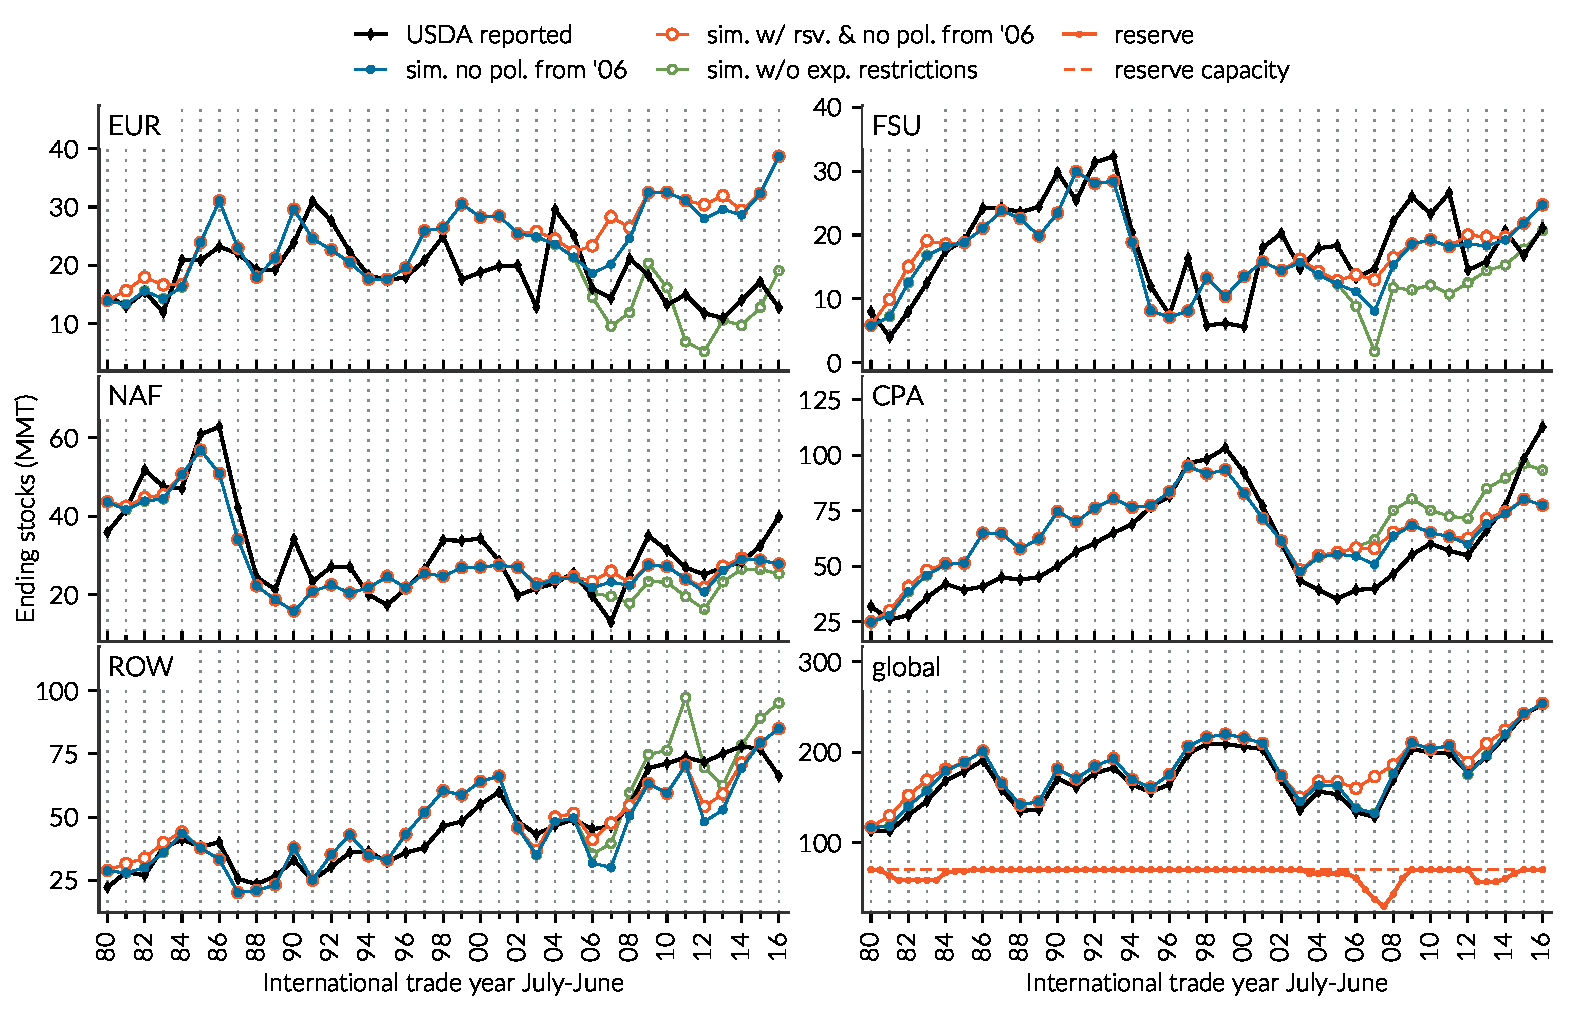
\includegraphics[width=.8\textwidth]{plots/no_policies_after_2006/Ending_stocks__MMT__1980_2017}
  \caption{Regional ending stock for the scenarios of Fig.~\ref{fig:prices_small_res}. Black
    diamonds, open green circles, blue dots, and open orange circles, indicate ending stocks as
    reported by USDA, for the scenario without export restrictions as well as the scenario without
    policy interventions from 2006 onwards (without and with international reserve),
    respectively. Parameters are as in Tab.~\ref{tab:params}. Regions are the same as in Tab.~\ref{tab:conGroup}.}
  \label{fig:stocks_small_res}
\end{figure}
This scenario describes, the optimal outcome of binding free-trade legislation impeding all kinds of
beggar-thy-neighbor policies after 2006. Thus, the factors $\lbrace m_r\rstu_r\rbrace_r$, describing
the regional demand for strategic stock-keeping are fixed to their 2006 levels for the international
trade years 2007 to 2016. Simulated prices and ending stocks resulting from this sceario are
depicted by open open orange circles in Figs.~\ref{fig:prices_small_res} and
\ref{fig:stocks_small_res}, respectively. In this scenario, a reserve of 30\mmt~would have been
sufficient to further mitigate the 2007/08 price spike (see filled open orange circles in
Figs.~\ref{fig:prices_small_res} and \ref{fig:stocks_small_res}). Since no consumption adaptation is
taken into account, the international reserve is initially filled to its capacity (see
discussion in main text.).

Further, the green dots in Figs.~\ref{fig:prices_small_res} and \ref{fig:stocks_small_res} depict a
scenario where only export restrictions are suppressed but the other policies are the same as in the
full historical scenario (cp. Figs.~\ref{fig:Fig1} and \ref{fig:Fig2}).

% \FloatBarrier

\subsection{Iso-elastic regional consumptions}
\begin{figure}[htbp]
  \centering
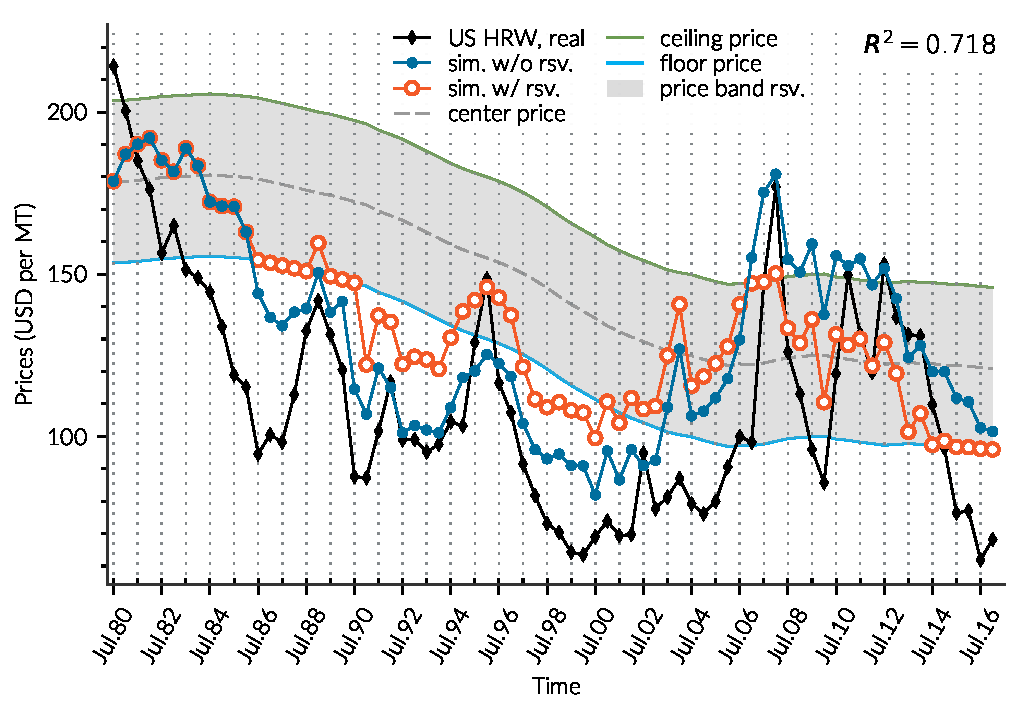
\includegraphics[width=.8\textwidth]{plots/full_var_demand/pric1980_2017}
\caption{Prices for the historical scenario with iso-elastic regional consumptions. Real wheat
  prices (black diamonds), simulated prices without (blue dots), and with a international reserve
  having a capacity of 70\mmt~(open orange circles). The gray shaded area indicates the price band
  of the international reserve; the reserve is re-stocked (released) if prices drop below (increase
  above) the floor price (thin light-blue line) (ceiling price (thin green line)). The price band
  has a width of 55\USD~and spans around the 15-years running mean (gray dashed line). The
  squared Pearson correlation coefficient $R^2$ denotes the correlation between reported prices and
  simulated prices (w/o reserve). Consumption elasticities are $\dce_{\CPA}=-0.1$, $\dce_{\ROW}=-0.05$, $\dce_{\EUR}=-0.15$, $\dce_{\FSU}=-0.5$, and $\dce_{\NAF}=-0.4$, and other parameters are as in
  Tab.~\ref{tab:params}.}
    \label{fig:varDem_price}
\end{figure}
\begin{figure}[htbp]
  \centering 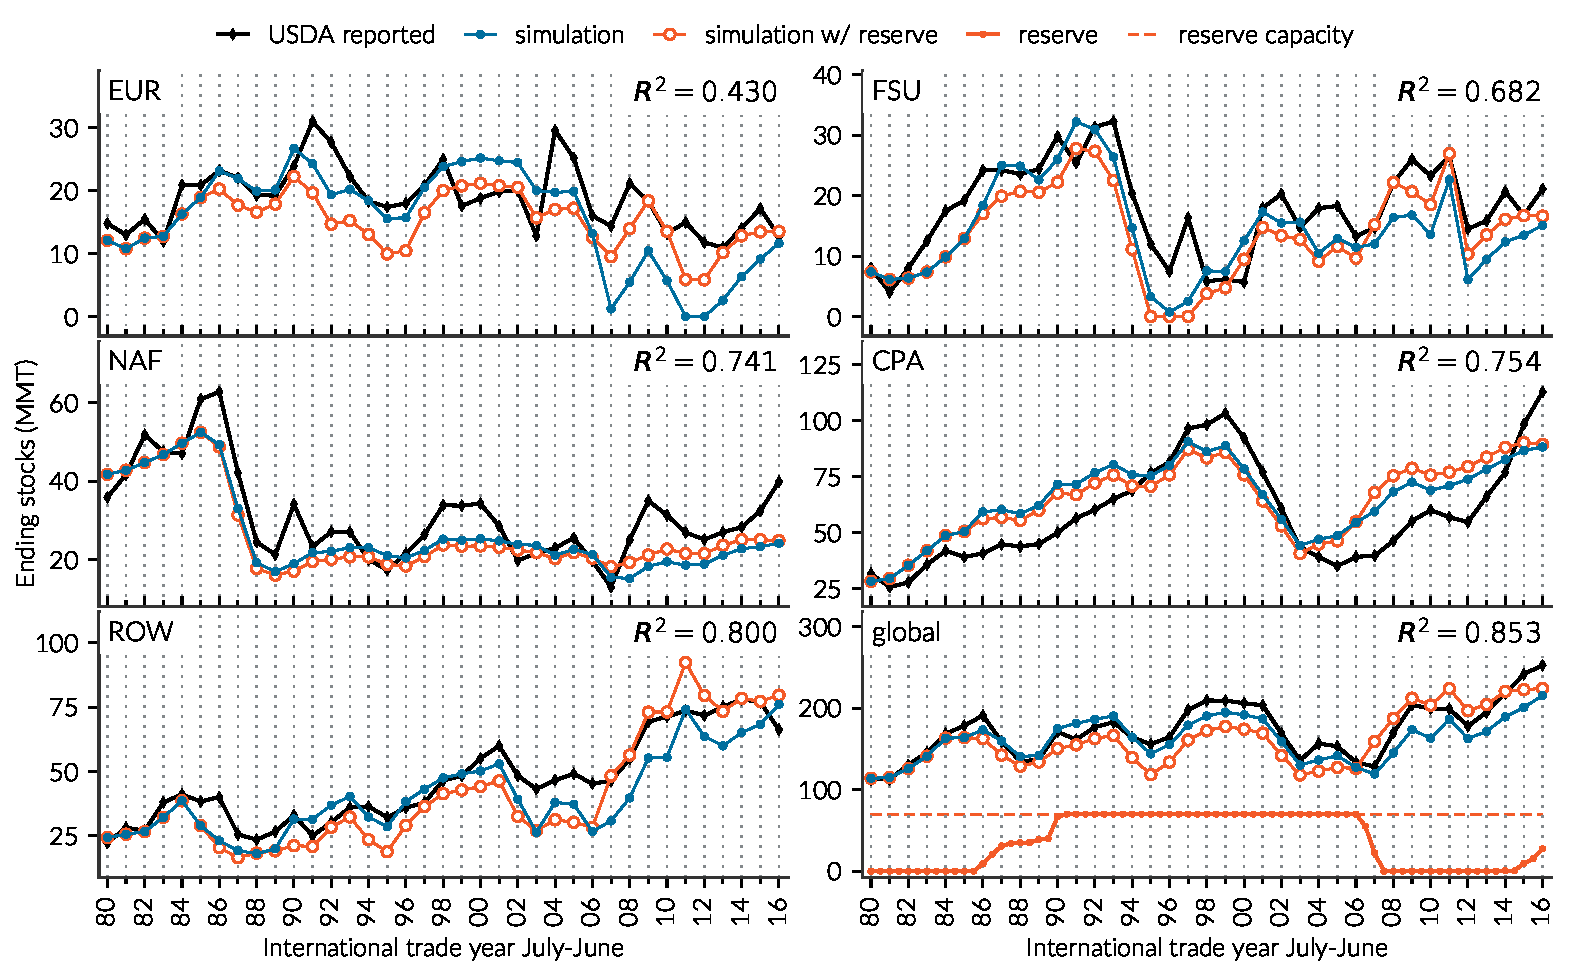
\includegraphics[width=.8\textwidth]{plots/full_var_demand/Ending_stocks__MMT__1980_2017}
  \caption{Regional ending stocks for the historical scenario with iso-elastic regional
    consumptions. Black diamonds, blue dots, and open orange circles, indicate ending stocks as
    reported by USDA, for the scenarios without and with international reserve,
    respectively. Squared Pearson correlation coefficients $R^2$ denote the correlation between
    reported stocks and the scenario without international reserve. Parameters are as in
    Fig.~\ref{fig:varDem_price}. Regions are the same as in Tab.~\ref{tab:conGroup}.}
    \label{fig:varDem_stocks}
\end{figure}
\begin{figure}[htbp]
  \centering  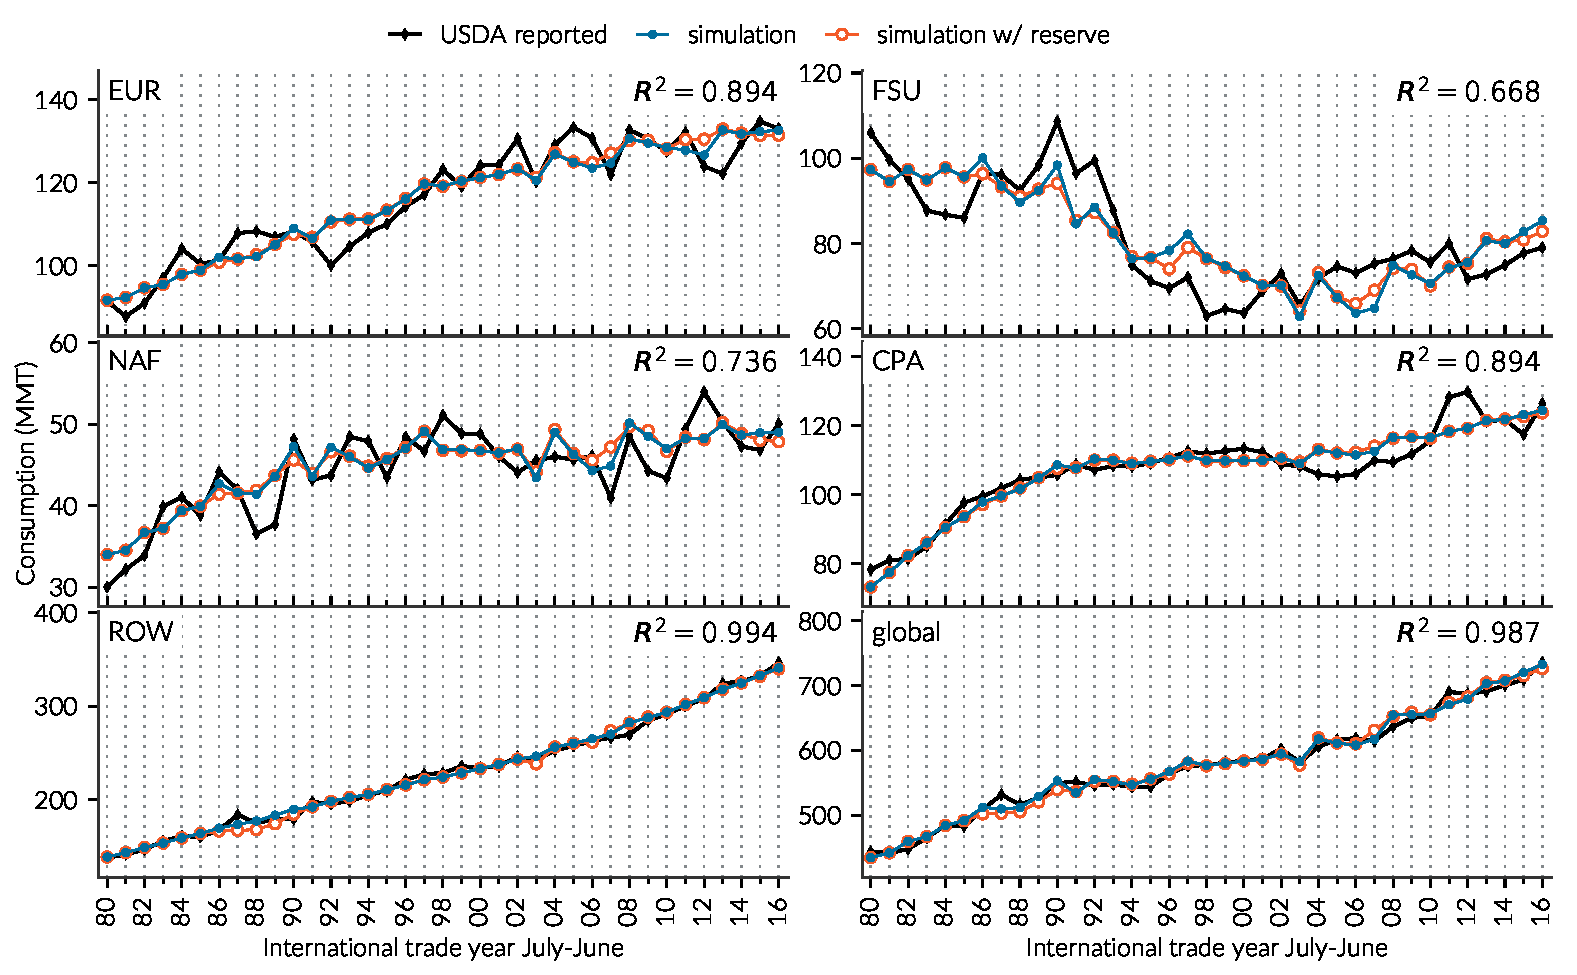
\includegraphics[width=.8\textwidth]{plots/full_var_demand/Consumption__MMT__1980_2017}
  \caption{Regional consumptions for the historical scenario with iso-elastic regional consumption. Color code is the same as in Fig.~\ref{fig:varDem_stocks}. Parameters are as in Fig.~\ref{fig:varDem_price}. Regions are the same as in Tab.~\ref{tab:conGroup}.}
  \label{fig:varDem_cons}
\end{figure}
This scenario corresponds to the full historic scenario described in the main text
(cf. Figs.~\ref{fig:Fig1} and \ref{fig:Fig2})) with the difference that now the regional
consumptions are assumed to depend iso-elastically upon WM price (see
Eq.~(\ref{eq:C_r})). Figures.~\ref{fig:varDem_price} and \ref{fig:varDem_stocks} compare simulated
WM prices and regional ending stocks with reported prices and ending stocks, respectively. The
elasticities of consumption vary among regions, which expresses the regions' different dependencies
upon the modeled crop. They are determined by best fit of simulated regional consumptions with
reported annual regional domestic consumption (see Fig.~\ref{fig:varDem_cons}) as
$\dce_{\CPA}=-0.1$, $\dce_{\ROW}=-0.05$, $\dce_{\EUR}=-0.15$, $\dce_{\FSU}=-0.5$, and $\dce_{\NAF}=-0.4$.  Further,
regional baseline consumption is determined from the average regional consumption of the last 3
years, $\Cref_r\equiv \langle C_r\rangle_3$, and the reference price is determined from the average
WM price of the last 3 years, $\Pref_r\equiv \langle \Pref_r\rangle_2$
(cf. Eq.~(\ref{eq:C_r})). In the initial steady state, the reference prices of all regions are set
to the reported WM price in the first semester of the international trade year.

Since, in this scenario, consumption adaption can be accounted for, the
reserve is chosen to be initially empty. Figure~\ref{fig:varDem_stocks} shows
that the build-up of the reserve has no significant negative impact on regional
endings stocks, and Fig.~\ref{fig:varDem_cons} reveals that regional domestic
consumption is only somewhat reduced. Thus, the negative impact of the reserve's build-up on vulnerable consumers is negligibly small.

% \FloatBarrier

\subsection{Statistical analysis}
\label{sec:artiTs}
This section provides details on the statistical analysis of Fig.~\ref{fig:Fig3}.

\paragraph{Initial conditions}
The simulations are initialized with the average regional productions and ending stocks of the
international trade years 2010 to 2015. Further, we use the average regional consumption of these
years to determine initial regional consumptions as described in Sec.~\ref{si:iniCond}. The initial
sizes of the strategical inventories $\lbrace \Ismax_r\rbrace_r$ are determined as described in
Sec.~\ref{si:iniCond}.

\paragraph{Artificial production time series}
Regional historical production anomalies are derived from USDA regional production data for the
international trade years 1965 to 2016 by de-trending with the smoothed data of Fig.~\ref{fig:supProd_and_cons}. The
artificial regional production time series having a length of 10,000 years are assembled by
randomly drawing, for each year and each region, a production anomaly out of the sample of
historical regional production anomalies. However, the results do not change qualitatively if the
regional anomalies are fitted by normal distributions, and the time series are generated by drawing
samples from these distributions. Further, regional baseline consumption $\Cref_r$ is determined
from the average regional consumption of the last 3 years, $\Cref_r\equiv \langle C_r\rangle_3$
(cf. Eq.~(\ref{eq:C_r})), and the reference price $\Pref_r$ is set to the average observed price of
the international trade years 2010 to 2015.

%%% Local Variables:
%%% mode: latex
%%% TeX-master: "multi_twist.tex"
%%% End:
